\subsection*{Partie A}

	\begin{enumerate}
		\item D'après l'énoncé, le point A$(0 ; 1)$ est sur la courbe représentative de $f$.

		On a donc :\quad $\begin{aligned}[t]
			f(0) = 1
				&\iff a + \dfrac{b\ln(0 + 1)}{0 + 1} = 1\\
				&\iff a + \dfrac{b\ln(1)}{1}= 1\\
				&\iff a = 1 \quad \text{car } \ln(1) = 0
		\end{aligned}$

		On a donc bien $a=1$.

		\item \begin{enumerate}
			\item La valeur de $f'(0)$ est le coefficient directeur de la tangente au point d'abscisse 0, c'est-à-dire de la tangente $T_{\mathrm{A}}$.

			Cette tangente passe par A et par B$(1 ; 5)$.

			Son coefficient directeur est donc :\quad $\dfrac{5 - 1}{1 - 0} = 4$.

			On a donc $f'(0) = 4$.

			\item Sur l'intervalle $[0 ; 2]$, au moins, la fonction $f$ est manifestement concave.

			Ainsi, on aura $f''$ à valeurs négatives sur au moins $[0 ; 2]$.

			Notamment, on a $f''(1)$ négatif.
		\end{enumerate}

		\item \begin{enumerate}
			\item $f$ est dérivable sur son ensemble de définition.

			Soit $x$ appartenant à $]-1 ;+\infty[$ :

			On peut dire que :\quad $x \longmapsto \ln(x + 1)$\quad a pour dérivée, par composition : \quad $x \longmapsto \dfrac{1}{x+1}$.

			Ainsi pour $x$ appartenant à $]-1 ;+\infty[$ :

			$f'(x)=0 + \dfrac{b \times \dfrac{1}{x+1}\times (x+1) - 1 \times b\ln(x+1)}{(x+1)^2}
			=\dfrac{b - b\ln(x+1)}{(x+1)^2} =
			\dfrac{b\big(1-\ln (x+1)\big)}{(x+1)^{2}}$

			\item D'après la question \textbf{2. a.}, on a $f'(0) = 4$.

			$\begin{aligned}
				f'(0) = 4
					&\iff \dfrac{b\big(1-\ln (0+1)\big)}{(0+1)^{2}} = 4\\
					&\iff \dfrac{b\big(1 - \ln(1)\big)}{1^2} = 4\\
					&\iff b(1 - 0) = 4\\
					&\iff b = 4
			\end{aligned}$

			On en déduit que \quad $b = 4$.
		\end{enumerate}
	\end{enumerate}

	\subsection*{Partie B}

	\begin{enumerate}
		\item D'après la propriété des croissances comparées :\quad $\lim\limits_{y \to +\infty} \dfrac{\ln(y)}{y} = 0$.

		Or :\quad $\lim\limits_{x \to +\infty} x+ 1 = + \infty$\quad donc, avec $y = x+1$, par composition, on en déduit :\quad $\lim\limits_{x \to +\infty} \dfrac{\ln(x+1)}{x+1} = 0$.

		Par limite de la somme et du produit :\quad $\lim\limits_{x \to +\infty} f(x) = \lim\limits_{x \to +\infty} 1 + 4\times \dfrac{\ln(x+1)}{x+1} = 1 + 4\times 0 = 1$.

		$f$ a une limite finie égale à 1, quand $x$ tend vers $+\infty$.

		Par définition, la droite d'équation \quad $y=1$ \quad est asymptote à la courbe représentative de la fonction~$f$ au voisinage de $+\infty$.

		\item Résolvons :\quad $\begin{aligned}[t]
			1-\ln (x+1)>0
				&\iff 1 > \ln(x+1)\\
				&\iff \e^{1} > x+1 \quad \text{car la fonction exp est strictement croissante sur }\R\\
				&\iff \e - 1 > x
		\end{aligned}$

		Sur $]-1 ;+\infty[$, l'ensemble des solutions de l'équation est $]-1 ; \e - 1[$.

		\item On a les limites de $f$ aux bornes de son ensemble de définition, l'une calculée à la question \textbf{1.}, l'autre admise.

		D'après la question \textbf{3. a.} de la \textbf{partie A}, on a, pour tout $x$ réel strictement supérieur à 1:

		$f'(x) = \dfrac{4\big(1 - \ln(x+1)\big)}{(x+1)^2} = \dfrac{4}{(x+1)^2} \times \big(1 - \ln(x+1)\big)$.

		Or :\quad $\forall x \in ]-1 ; +\infty[,\quad \dfrac{4}{(x+1)^2} > 0$

		Pour tout $x$ strictement supérieur à 1, le signe du nombre dérivé $f'(x)$ est donc donné par le signe de l'expression \quad$1 - \ln(x+1)$.

		On a établi ce signe à la question précédente.

		Le changement de variations de $f$ interviendra donc pour $x = \e - 1$.

		$f(\e - 1) = 1 + \dfrac{4\ln(\e - 1 + 1)}{\e - 1 + 1} = 1 + \dfrac{4\ln(\e)}{\e}= 1 + \dfrac{4}{\e} = 1 + 4\e^{-1}$.

		On a donc le tableau de variation complet de la fonction $f$ :

		\begin{center}
			\begin{tikzpicture}
			\tkzTabInit[lgt=3,espcl=4]{$x$/0.7, signe de $f'(x)$/0.7, variations de $f$/2.5}
			{$-1$,$\e -1$, $+\infty$}
			\tkzTabLine{d,+,z,-,}
			\tkzTabVar{D-/$-\infty$,+/$1 + 4\e^{-1}$,-/$1$}
		\end{tikzpicture}
		\end{center}

		\item $\e$ est inférieur à 3, donc $\e - 1$ est inférieur à 2 (on a : $\e - 1 \approx 1,72$).

		Sur l'intervalle $[2 ; +\infty[$, $f$ est continue (car dérivable) et strictement décroissante.

		De plus 1,5 est une valeur intermédiaire entre \quad $f(2) = 1 + \dfrac{4\ln(3)}{3} \approx 2,46$ \quad et \quad$\lim\limits_{x \to +\infty} f(x) = 1$.

		D'après le corollaire au théorème des valeurs intermédiaires appliqué aux fonctions strictement monotones (dit aussi théorème de la bijection), l'équation \quad $f(x)=1,5$ \quad admet une unique solution dans l'intervalle $[2 ; +\infty[$.

		À la calculatrice, on obtient 25,1 comme valeur approchée arrondie à $10^{-1}$ de cette solution.

		\item \begin{enumerate}
			\item Posons $u$ définie sur $]-1 ; +\infty[$ par :\quad $u : x \longmapsto \ln(x+1)$.

			On a :\quad $u' : x \longmapsto \dfrac{1}{x+1}$.

			On reconnaît donc, pour tout $x$ dans $[0 ; 2]$ :\quad $\dfrac{\ln(x+1)}{x+1} = \ln(x+1) \times \dfrac{1}{x+1} = u(x) \times u'(x)$.

			On en déduit :
			$\begin{aligned}[t]
				\int_{0}^{2} \dfrac{\ln (x+1)}{x+1} \d{}x
					&= \left[\dfrac{1}{2}\big(\ln(x+1)\big)^2\right]_{0}^{2}\\
					&= \left(\dfrac{1}{2}\big(\ln(2+1)\big)^2\right) - \left(\dfrac{1}{2}\big(\ln(0+1)\big)^2\right)\\
					&= \dfrac{1}{2}\big(\ln 3\big)^{2} - \dfrac{1}{2}\big(\ln 1\big)^{2}\\
					&=\dfrac{1}{2}\big(\ln 3\big)^{2} \quad \text{car } \ln(1) = 0
			\end{aligned}$

			\item Comme la fonction $f$ est une fonction continue et positive sur $[0 ; 2]$, l'aire, en unité d'aire, du domaine délimité par l'axe des abscisses, la courbe représentative de la fonction $f$, l'axe des ordonnées et la droite d'équation \quad $x=2$ correspond à :\quad $\ds \mathcal{A} = \int_{0}^{2} f(x) \d x$.

			$\begin{aligned}
				\ds \mathcal{A} = \int_{0}^{2} f(x) \d x
					& = \int_{0}^{2} \left(1 + \dfrac{4\ln(x+1)}{x+1}\right) \d x\\
					& = \int_{0}^{2} 1\d x + 4 \int_{0}^{2} \dfrac{\ln(x+1)}{x+1} \d x \quad \text{par linéarité de l'intégrale}\\
					& = 2 + 4 \times \dfrac{1}{2}\big(\ln 3\big)^{2} \quad \text{d'après la question précédente}\\
					& = 2 + 2\big(\ln 3\big)^{2}
			\end{aligned}$

			En unité d'aire, l'aire demandée est donc $2 + 2\big(\ln 3\big)^{2}$
		\end{enumerate}
	\end{enumerate}
